\documentclass{article}
\usepackage{graphicx} % Add the graphicx package for including images


\title{Mercedes AMG Bobby Car \\ Requirements Document}
\date{\today}

\begin{document}
	
	\maketitle
	
	\tableofcontents % Add a table of contents
	
	\newpage
	
	\section{Customer Requirements}
	
	\begin{figure}[h!] % Place the image in a figure environment with [h] for placement "here"
		\centering % Center the image
		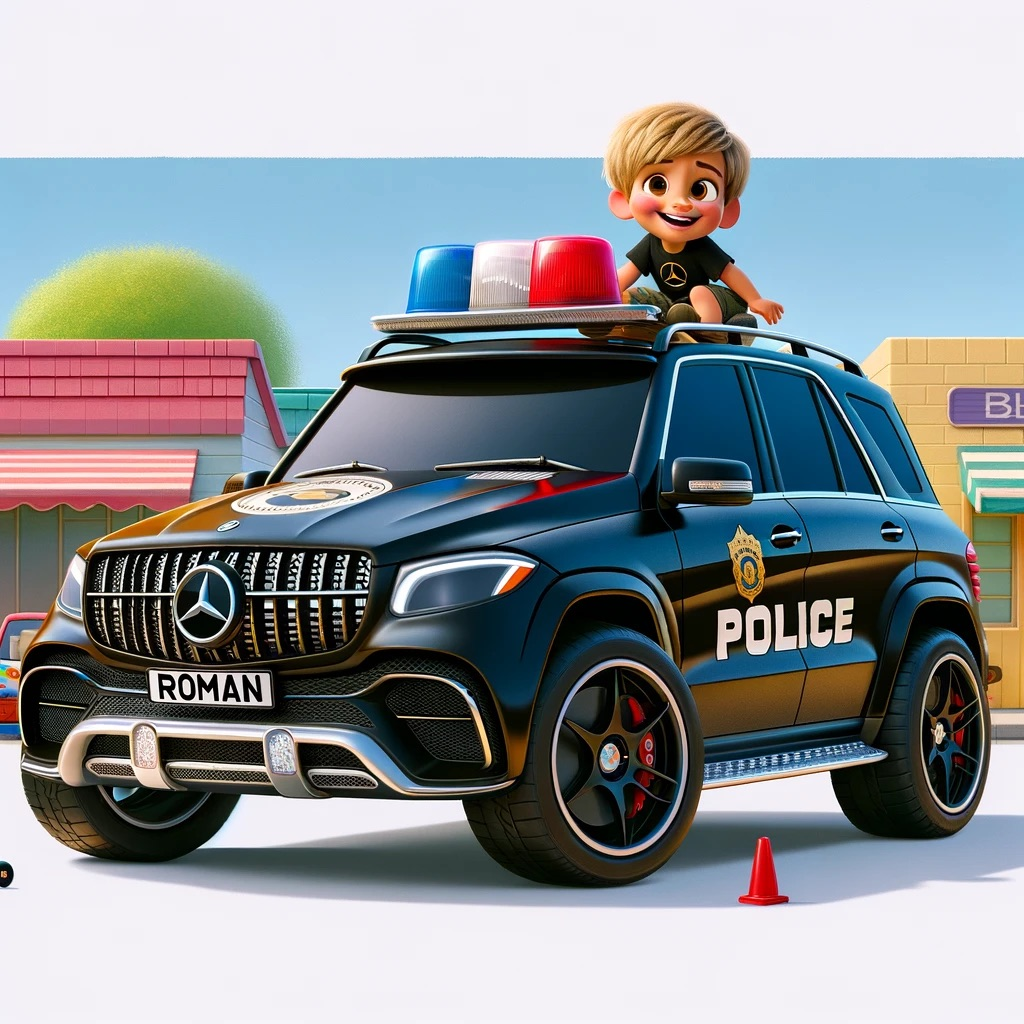
\includegraphics[width=1.0\textwidth]{Customer_View.jpeg} % Adjust the width as needed
		\caption{Customer Level Requirements}
	\end{figure}
	
	\subsection{Requirement CR001: Replace Mercedes AMG Bobby Car "Entertainment System"}
	\begin{itemize}
		\item \textbf{Description:} The system shall replace the existing Mercedes AMG Bobby Car "Entertainment System" with a new modern "Entertainment System."
		\item \textbf{Priority:} High
		\item \textbf{Source:} Parents of the Child
		\item \textbf{Acceptance Criteria:}
		\begin{itemize}
			\item The old Entertainment System is not active anymore.
			\item The new Entertainment System has distinct sensory characteristics, providing a different feel and sound compared to the old one.
		\end{itemize}
		\item \textbf{Dependencies:} None
	\end{itemize}
	
	\subsection{Requirement CR002: Music and Audiobook Player Integration}
	\begin{itemize}
		\item \textbf{Description:} The system shall be able to play songs from Spotify and play audiobooks from Audible.
		\item \textbf{Priority:} Low
		\item \textbf{Source:} Parents of the Child
		\item \textbf{Acceptance Criteria:}
		\begin{itemize}
			\item Users can select a song from Spotify.
			\item Users can select an audiobook from Audible.
		\end{itemize}
		\item \textbf{Dependencies:} None
	\end{itemize}
	
	\subsection{Requirement CR004: Martinshorn Siren Sound}
	\begin{itemize}
		\item \textbf{Description:} The system shall be able to play the siren sound of a German police car or a firefighter car.
		\item \textbf{Priority:} High
		\item \textbf{Source:} Child
		\item \textbf{Acceptance Criteria:}
		\begin{itemize}
			\item Users can activate the Martinshorn (siren).
			\item Users can hear the Martinshorn.
		\end{itemize}
		\item \textbf{Dependencies:} None
	\end{itemize}
	
	\subsection{Requirement CR005: Exterior Light Blinking}
	\begin{itemize}
		\item \textbf{Description:} The system shall be able to control the existing exterior lights of the Mercedes AMG Bobby Car.
		\item \textbf{Priority:} High
		\item \textbf{Source:} Child
		\item \textbf{Acceptance Criteria:}
		\begin{itemize}
			\item Users can enjoy blinking exterior lights if one of the functions is active.
		\end{itemize}
		\item \textbf{Dependencies:} None
	\end{itemize}
	
	\subsection{Requirement CR006: Simulate Engine Start}
	\begin{itemize}
		\item \textbf{Description:} The system shall simulate the engine start of the real Mercedes AMG car.
		\item \textbf{Priority:} High
		\item \textbf{Source:} Child
		\item \textbf{Acceptance Criteria:}
		\begin{itemize}
			\item Users can start the imaginary engine of the AMG Bobby Car.
		\end{itemize}
		\item \textbf{Dependencies:} None
	\end{itemize}
	
	\subsection{Requirement CR007: Battery Life}
	\begin{itemize}
		\item \textbf{Description:} The system shall work without an external power supply for a minimum of 12 hours.
		\item \textbf{Priority:} High
		\item \textbf{Source:} Parents of the Child
		\item \textbf{Acceptance Criteria:}
		\begin{itemize}
			\item Users can use all functions for 12 hours.
		\end{itemize}
		\item \textbf{Dependencies:} None
	\end{itemize}
	
	\subsection{Requirement CR008: Remote Control Functionality}
	\begin{itemize}
		\item \textbf{Description:} The system shall provide a remote control for volume control, song switching, engine start, and Martinshorn activation.
		\item \textbf{Priority:} Middle
		\item \textbf{Source:} Parents of the Child
		\item \textbf{Acceptance Criteria:}
		\begin{itemize}
			\item Users can change the volume level remotely.
			\item Users can change the song remotely.
			\item Users can start or stop the Martinshorn remotely.
		\end{itemize}
		\item \textbf{Dependencies:} The functions mentioned (volume control, song switching, engine start, and Martinshorn activation) must be implemented for onboard control.
	\end{itemize}
	
	\subsection{Requirement CR009: Safety Features}
	\begin{itemize}
		\item \textbf{Description:} The system shall have safety mechanisms to prevent unintended acceleration, including a safety lock for unsupervised usage and an emergency stop feature.
		\item \textbf{Priority:} Middle
		\item \textbf{Source:} Safety Standards
		\item \textbf{Acceptance Criteria:}
		\begin{itemize}
			\item The safety mechanisms prevent unintended acceleration.
			\item The emergency stop feature halts the vehicle immediately when activated.
		\end{itemize}
	\end{itemize}
	
	\subsection{Requirement CR010: User Interface and Accessibility}
	\begin{itemize}
		\item \textbf{Description:} The system shall have an intuitive and user-friendly interface suitable for children, support multiple languages, and provide audio or visual cues for users with disabilities.
		\item \textbf{Priority:} Middle
		\item \textbf{Source:} User Experience
		\item \textbf{Acceptance Criteria:}
		\begin{itemize}
			\item The interface is user-friendly for children.
			\item The system supports multiple languages.
			\item It provides cues for users with disabilities.
		\end{itemize}
	\end{itemize}
	
	\subsection{Requirement CR011: Battery Management}
	\begin{itemize}
		\item \textbf{Description:} The system shall include a low battery warning indicator, a battery charging and monitoring system, and automatic shutdown or low-power mode when the battery is critically low.
		\item \textbf{Priority:} Middle
		\item \textbf{Source:} System Design
		\item \textbf{Acceptance Criteria:}
		\begin{itemize}
			\item The low battery warning indicator functions as intended.
			\item The battery charging and monitoring system is effective.
			\item Automatic shutdown/low-power mode activates when the battery is critically low.
		\end{itemize}
	\end{itemize}
	
	\subsection{Requirement CR012: Remote Monitoring and Parental Control}
	\begin{itemize}
		\item \textbf{Description:} The system shall allow parents to monitor the vehicle's location and speed remotely and provide parental control options to limit speed or functionality based on the child's age or skill level.
		\item \textbf{Priority:} Middle
		\item \textbf{Source:} Parental Requirements
		\item \textbf{Acceptance Criteria:}
		\begin{itemize}
			\item Parents can monitor the vehicle's location and speed remotely.
			\item Parental control options are available and function as specified.
		\end{itemize}
	\end{itemize}
	
	\subsection{Requirement CR013: Data Privacy and Security}
	\begin{itemize}
		\item \textbf{Description:} The system shall ensure the privacy and security of user data, especially when connected to external services like Spotify or Audible.
		\item \textbf{Priority:} Middle
		\item \textbf{Source:} Data Privacy Standards
		\item \textbf{Acceptance Criteria:}
		\begin{itemize}
			\item User data is securely protected, especially when connected to external services.
		\end{itemize}
	\end{itemize}
	
	\subsection{Requirement CR014: Compliance with Regulations}
	\begin{itemize}
		\item \textbf{Description:} The system shall adhere to safety and regulatory standards applicable to children's toys and vehicles in your region.
		\item \textbf{Priority:} High
		\item \textbf{Source:} Regulatory Standards
		\item \textbf{Acceptance Criteria:}
		\begin{itemize}
			\item The system complies with all relevant safety and regulatory standards.
		\end{itemize}
	\end{itemize}
	
	\subsection{Requirement CR015: Durability and Weather Resistance}
	\begin{itemize}
		\item \textbf{Description:} The system shall be designed to withstand various weather conditions and resist damage from outdoor use.
		\item \textbf{Priority:} Middle
		\item \textbf{Source:} Durability Standards
		\item \textbf{Acceptance Criteria:}
		\begin{itemize}
			\item The system remains operational and undamaged after exposure to various weather conditions and outdoor use.
		\end{itemize}
	\end{itemize}
	
	\subsection{Requirement CR016: User Manual and Documentation}
	\begin{itemize}
		\item \textbf{Description:} The system shall come with a comprehensive user manual for setup, operation, and maintenance.
		\item \textbf{Priority:} Middle
		\item \textbf{Source:} User Experience
		\item \textbf{Acceptance Criteria:}
		\begin{itemize}
			\item A comprehensive user manual is provided with clear instructions for setup, operation, and maintenance.
		\end{itemize}
	\end{itemize}
	
	\subsection{Requirement CR017: Product Warranty}
	\begin{itemize}
		\item \textbf{Description:} The system shall include a warranty period and terms for repairs or replacements.
		\item \textbf{Priority:} Middle
		\item \textbf{Source:} Customer Support
		\item \textbf{Acceptance Criteria:}
		\begin{itemize}
			\item The product warranty period and terms are clearly stated and provided to customers.
		\end{itemize}
	\end{itemize}

	\newpage

	\section{System Requirements}	
	
	\begin{figure}[h!] % Place the image in a figure environment with [h] for placement "here"
		\centering % Center the image
		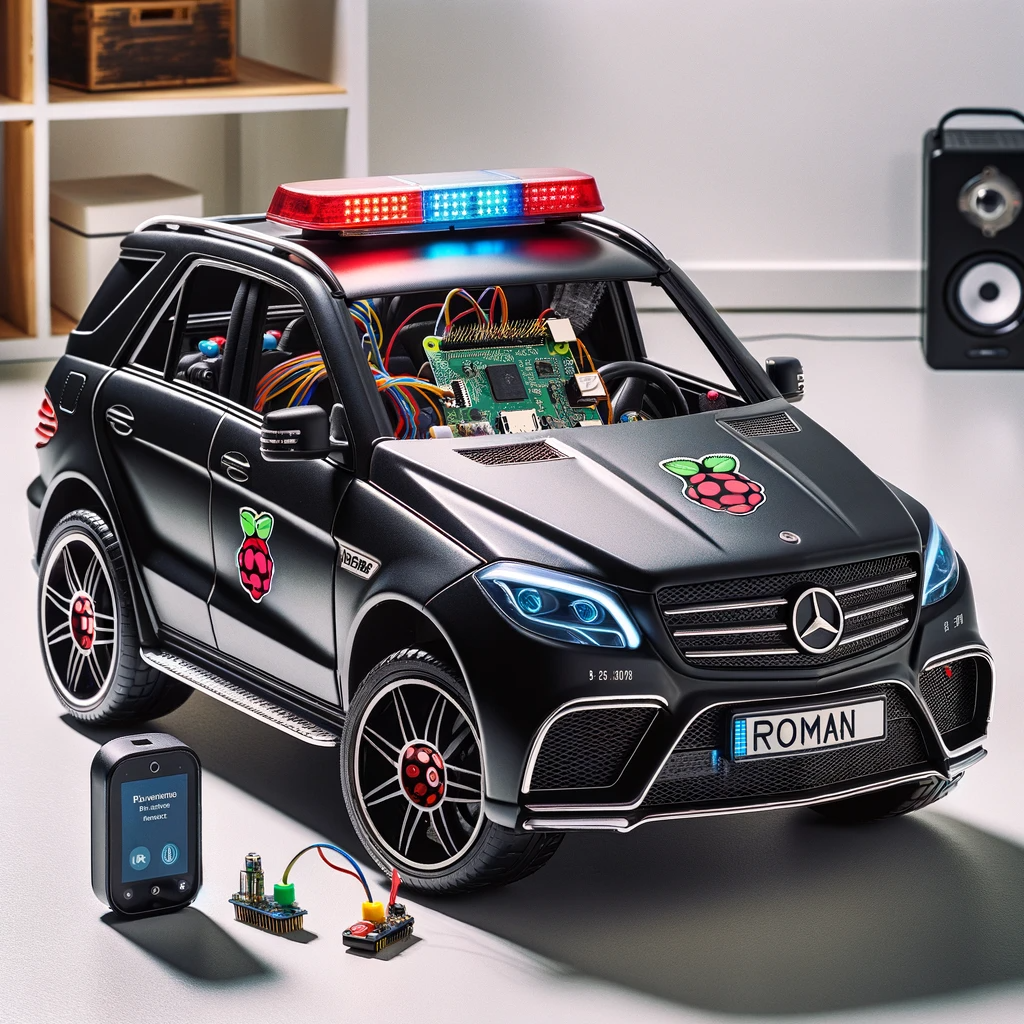
\includegraphics[width=1.0\textwidth]{System_View.png} % Adjust the width as needed
		\caption{System Level Requirements}
	\end{figure}
	
	
\end{document}
